\documentclass[a4paper, 11pt]{article}

%% ─── Packages ───────────────────────────────────────────────────────────────
\usepackage[utf8]{inputenc}
\usepackage[T1]{fontenc}
\usepackage[french]{babel}
\usepackage{amsmath, amssymb}
\usepackage{siunitx}
\usepackage{booktabs}
\usepackage{graphicx}
\usepackage{hyperref}
\usepackage{geometry}
\usepackage{multicol}
\usepackage{fancyhdr}
\usepackage{titlesec}
\usepackage{enumitem}
\usepackage{caption}
\usepackage{float}
\usepackage{array}
\usepackage{xcolor}
\geometry{margin=2.5cm, top=3cm}
\sisetup{locale=FR, uncertainty-mode=separate, per-mode=symbol}

%% ─── En-tête / pied de page ─────────────────────────────────────────────────
\pagestyle{fancy}
\fancyhf{}
\lhead{Physique 4 – MT2 \textbar{} Labo 4A}
\rhead{HEPIA – HES-SO Genève}
\cfoot{\thepage}

%% ─── Macros pratiques ───────────────────────────────────────────────────────
\newcommand{\foc}{f}                % distance focale
\newcommand{\pobj}{p}               % distance objet
\newcommand{\qimg}{q}               % distance image

%% ─── Titre ──────────────────────────────────────────────────────────────────
\title{\textbf{Laboratoire 4A}\\[4pt]
       \large Lentilles minces et instruments d'optique}
\author{[Ton nom] \and Guilhem Rozier Vilardell \and [autres coéquipiers]}
\date{MT2 -- Semestre de printemps 2026}

%% ═══════════════════════════════════════════════════════════════════════════
\begin{document}
\maketitle
\tableofcontents
\newpage

%% ───────────────────────────────────────────────────────────────────────────
\section{Introduction}

Ce laboratoire porte sur la formation d'image par des lentilles minces et sur la construction d'un microscope expérimental. Les objectifs sont~:
\begin{itemize}
  \item vérifier expérimentalement la relation de conjugaison de Gauss ;
  \item déterminer la focale d'une lentille inconnue par la méthode de Bessel ;
  \item analyser le comportement de systèmes centrés à deux lentilles (convergentes, divergentes, accolées) ;
  \item mesurer le grossissement d'un microscope à deux lentilles et le comparer à la théorie.
\end{itemize}

%% ───────────────────────────────────────────────────────────────────────────
\section{Rappels théoriques}

\subsection{Formule de Gauss et grandissement}

Pour une lentille mince de distance focale $f$, la relation de conjugaison (formule de Gauss) entre la distance objet $p$ et la distance image $q$ est~:
\begin{equation}
  \frac{1}{p} + \frac{1}{q} = \frac{1}{f}
  \label{eq:gauss}
\end{equation}
avec la convention de signe : $p>0$ pour un objet réel, $q>0$ pour une image réelle.

Le grandissement transversal est défini par~:
\begin{equation}
  \gamma = \frac{\overline{A_1B_1}}{\overline{AB}} = -\frac{q}{p}
  \label{eq:grandissement}
\end{equation}
Il est négatif pour une image renversée (image réelle d'un objet réel par une lentille convergente).

\subsection{Méthode de Bessel}

Pour un écran et un objet fixés à une distance $D$, il existe deux positions de la lentille donnant une image nette, séparées par une distance $d$. On montre que~:
\begin{equation}
  f = \frac{D^2 - d^2}{4D}
  \label{eq:bessel}
\end{equation}
Cette méthode élimine le besoin de connaître la position exacte du centre optique de la lentille.

\subsection{Focale équivalente de deux lentilles accolées}

Deux lentilles de focales $f_1$ et $f_2$ placées en contact ($d \to 0$) se comportent comme une lentille unique de focale~:
\begin{equation}
  \frac{1}{f} = \frac{1}{f_1} + \frac{1}{f_2}
  \label{eq:lentilles_accolees}
\end{equation}

\subsection{Grossissement du microscope}

Le grossissement commercial d'un microscope (distance minimale de vision distincte $d_m = \SI{250}{mm}$) est~:
\begin{equation}
  G_c = \Phi \cdot d_m = \frac{\Delta}{f_\mathrm{ob}\,f_\mathrm{oc}} \cdot d_m
  \label{eq:grossissement}
\end{equation}
où $\Delta$ est la longueur optique (distance entre le foyer image de l'objectif $F'_1$ et le foyer objet de l'oculaire $F_2$), $f_\mathrm{ob}$ la focale de l'objectif et $f_\mathrm{oc}$ la focale de l'oculaire.

%% ───────────────────────────────────────────────────────────────────────────
\section{Questions préliminaires}

\subsection*{a) Démonstration de la formule de Bessel (éq.~\ref{eq:bessel})}

Soit $O_1$ et $O_2$ les deux positions de la lentille. Pour $O_1$~: $p_1 + q_1 = D$ et, pour $O_2$ (par symétrie) $p_2 = q_1$, $q_2 = p_1$. La distance entre les positions vaut $d = |p_1 - q_1|$. On a donc~:
\begin{align*}
  D &= p_1 + q_1, \quad d = p_1 - q_1 \quad (p_1 > q_1) \\
  \Rightarrow\; p_1 &= \frac{D+d}{2}, \quad q_1 = \frac{D-d}{2}
\end{align*}
En substituant dans $1/p_1 + 1/q_1 = 1/f$~:
\begin{equation*}
  f = \frac{p_1\,q_1}{p_1+q_1} = \frac{\dfrac{D+d}{2}\cdot\dfrac{D-d}{2}}{D} = \frac{D^2-d^2}{4D}
\end{equation*}

\textbf{Autres méthodes~:} On peut aussi utiliser (i) la méthode directe (mesure de $p$ et $q$ puis régression sur $1/p + 1/q = 1/f$) ou (ii) l'image à l'infini ($f = p$ quand $q \to \infty$). La méthode de Bessel est plus précise que la méthode directe car elle ne nécessite pas de localiser l'origine optique de la lentille.

\subsection*{b) Focale équivalente de deux lentilles accolées}

La relation de Gauss pour $L_1$~: $1/q_1 = 1/f_1 - 1/p$. Pour $d=0$, $p_2 = -q_1$ (l'image de $L_1$ devient l'objet de $L_2$, virtuel si $q_1 > 0$). La relation pour $L_2$~:
\begin{equation*}
  \frac{1}{q_\mathrm{tot}} = \frac{1}{f_2} - \frac{1}{p_2} = \frac{1}{f_2} + \frac{1}{q_1} = \frac{1}{f_2} + \frac{1}{f_1} - \frac{1}{p}
\end{equation*}
Donc $1/q_\mathrm{tot} + 1/p = 1/f_1 + 1/f_2 = 1/f_\mathrm{eq}$, ce qui démontre l'équation~\eqref{eq:lentilles_accolees}.

\subsection*{c) Construction de l'image pour un système à deux lentilles}

On applique la méthode en deux étapes~:
\begin{enumerate}
  \item Construire l'image $A_1B_1$ de $AB$ par $L_1$ seule (trois rayons remarquables).
  \item Utiliser $A_1B_1$ comme objet pour $L_2$, en calculant $p_2$ à partir de la position de $A_1B_1$ et de la séparation $d$ entre les lentilles~: $p_2 = d - q_1$.
\end{enumerate}

%% ───────────────────────────────────────────────────────────────────────────
\section{Dimensionnement}

\subsection*{a) Tracé des rayons – lentille convergente et divergente}

Pour une lentille convergente ($f>0$), les deux méthodes sont~:
\begin{enumerate}[label=\textbf{M\arabic*.}]
  \item Rayon passant par le centre optique~: aucune déviation. Rayon parallèle à l'axe~: passe par $F'$.
  \item Rayon quelconque vers le foyer objet $F$~: ressort parallèle à l'axe. Intersection des deux rayons émergents $\to$ point image.
\end{enumerate}
Pour une lentille divergente ($f<0$), mêmes constructions mais $F'$ est \emph{virtuel} (côté objet).

\subsection*{b) Calculs pour $f = \SI{100}{mm}$, $AB = \SI{16}{mm}$}

\textbf{Image $\times 4$ plus grande~:} $|\gamma| = 4 \Rightarrow q/p = 4 \Rightarrow q = 4p$. En substituant dans~\eqref{eq:gauss}~:
\begin{equation*}
  \frac{1}{p} + \frac{1}{4p} = \frac{1}{100\,\mathrm{mm}} \implies p = \frac{5}{4}\cdot 100 = \SI{125}{mm}, \quad q = \SI{500}{mm}
\end{equation*}

\textbf{Image $\times 3$ plus petite~:} $|\gamma| = 1/3 \Rightarrow q = p/3$.
\begin{equation*}
  \frac{1}{p} + \frac{3}{p} = \frac{1}{100\,\mathrm{mm}} \implies p = \SI{400}{mm}, \quad q = \SI{133}{mm}
\end{equation*}

\textbf{Distance sans image~:} Aucune image réelle n'existe pour $p \leq f$, c'est-à-dire $p \leq \SI{100}{mm}$ (objet dans ou au-delà du plan focal objet).

\subsection*{Dimensionnement microscope}

Objectif~: $f_\mathrm{ob} = \SI{2}{mm}$, oculaire~: $f_\mathrm{oc} = \SI{25}{mm}$, longueur optique $\Delta = \SI{160}{mm}$, $d_m = \SI{250}{mm}$.
\begin{align*}
  \Phi &= \frac{\Delta}{f_\mathrm{ob}\,f_\mathrm{oc}} = \frac{160}{2\times 25} = \SI{3.2}{mm^{-1}} = \SI{3200}{dioptries} \\
  G_c  &= \Phi\,d_m = 3.2 \times 250 = 800
\end{align*}

%% ───────────────────────────────────────────────────────────────────────────
\section{Manipulation 1a – Relation de conjugaison de Gauss}

\subsection{Protocole}

Une lentille convergente de focale nominale $f = \SI{100}{mm}$ est placée sur un banc optique. L'objet est un diaphragme en forme de «~F~» éclairé par une LED collimatée. Pour 10 valeurs de $p$ (distance objet–lentille), on cherche la position de l'écran donnant une image nette et on mesure~: $p$, $q$ et la taille $\overline{A_1B_1}$ de l'image.

Correction de zéro (offsets mesurés indépendamment)~: $p = p_\text{brut} + \SI{17}{mm}$ et $q = q_\text{brut} - \SI{5}{mm}$. Taille nominale de l'objet~: $\overline{AB} = \SI{10}{mm}$. Incertitudes~: $u(p) = \sqrt{2} \approx \SI{1.41}{mm}$, $u(q) = \sqrt{5} \approx \SI{2.24}{mm}$ (lecture image $\pm\SI{2}{mm}$, offset $\pm\SI{1}{mm}$), $u(\overline{A_1B_1}) = \SI{1}{mm}$.

\subsection{Données expérimentales}

\begin{table}[H]
\centering
\caption{Données corrigées et grandissements – Manipulation 1a ($f_\mathrm{nom} = \SI{100}{mm}$)}
\label{tab:1a_brut}
\begin{tabular}{rrrrll}
\toprule
$p$ (mm) & $q$ (mm) & $\overline{A_1B_1}$ (mm) & $|\gamma|$ & $1/q$ (\si{10^{-3}.mm^{-1}}) & $-1/p$ (\si{10^{-3}.mm^{-1}}) \\
\midrule
115 & 645 & 55 & 5.5 & 1.550 & $-$8.696 \\
125 & 459 & 36 & 3.6 & 2.179 & $-$8.000 \\
130 & 388 & 30 & 3.0 & 2.577 & $-$7.692 \\
135 & 349 & 25 & 2.5 & 2.865 & $-$7.407 \\
140 & 326 & 23 & 2.3 & 3.067 & $-$7.143 \\
145 & 304 & 21 & 2.1 & 3.289 & $-$6.897 \\
150 & 280 & 19 & 1.9 & 3.571 & $-$6.667 \\
155 & 272 & 18 & 1.8 & 3.676 & $-$6.452 \\
160 & 245 & 16 & 1.6 & 4.082 & $-$6.250 \\
165 & 238 & 15 & 1.5 & 4.202 & $-$6.061 \\
\bottomrule
\end{tabular}
\end{table}

\subsection{Résultats de la régression linéaire}

La relation de conjugaison~\eqref{eq:gauss} se réécrit~:
\begin{equation}
  \frac{1}{q} = -\frac{1}{p} + \frac{1}{f}
  \label{eq:gauss_lin}
\end{equation}
ce qui correspond à une droite de pente $m = 1$ et d'ordonnée à l'origine $b = 1/f$.

La régression linéaire $1/q = m \cdot (-1/p) + b$ donne~:
\begin{align}
  m &= \num{1.0054} \pm \num{0.0246} \qquad (\text{attendu~: } +1) \notag\\
  b &= \SI{10.271e-3}{mm^{-1}} \pm \SI{0.176e-3}{mm^{-1}} \notag\\
  R^2 &= \num{0.99524} \notag\\
  f &= 1/b = \SI{97.4 \pm 1.7}{mm}
  \label{eq:f_1a}
\end{align}

\begin{figure}[H]
  \centering
  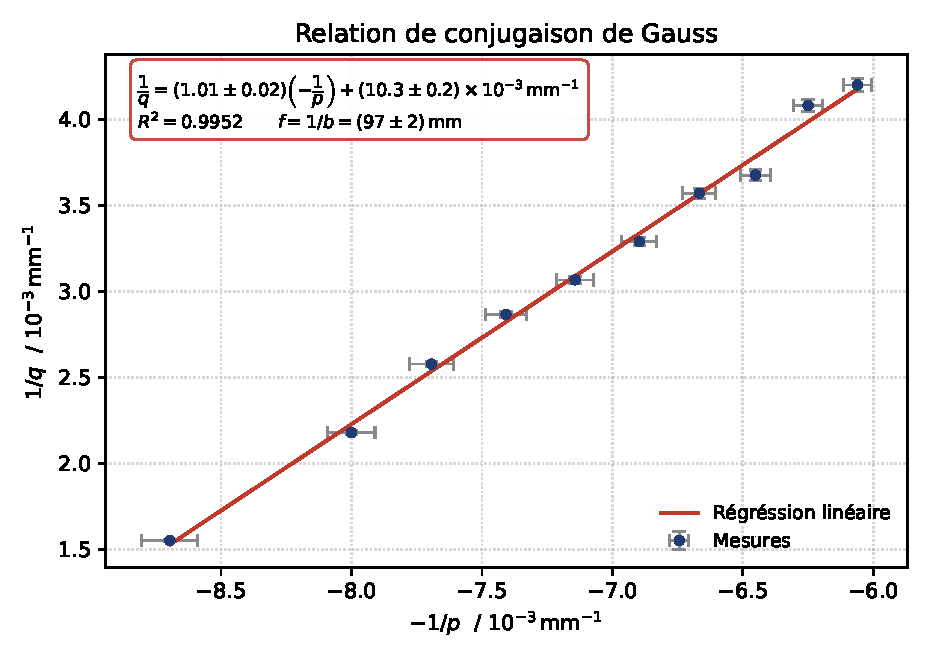
\includegraphics[width=0.72\textwidth]{labo4_1a_gauss.pdf}
  \caption{Régression $1/q$ vs $-1/p$ (manip 1a). La pente $m = \num{1.005}$ est compatible avec la valeur théorique $+1$ ; l'ordonnée à l'origine donne $f = 1/b = \SI{97.4}{mm}$.}
  \label{fig:1a_gauss}
\end{figure}

\subsection{Discussion}

\textbf{Coefficient directeur~:} La pente $m = \num{1.005} \pm \num{0.025}$ est compatible avec la valeur théorique $+1$ (écart relatif $\SI{0.5}{\percent}$, soit $\sim 0{,}2\sigma$). La relation de conjugaison de Gauss est donc vérifiée~: l'échange objet/image laisse la droite $1/q$ vs $-1/p$ de pente unité.

\textbf{Focale estimée~:} $f = 1/b = \SI{97.4 \pm 1.7}{mm}$, à comparer à la valeur nominale $\SI{100}{mm}$ (écart relatif $\SI{2.6}{\percent}$). L'écart de $\SI{2.6}{mm}$ ($\sim 1{,}6\,\delta f$) est expliqué par~:
\begin{itemize}
  \item les incertitudes de lecture des positions et la localisation du plan image net~;
  \item une tolérance de fabrication sur la focale réelle de la lentille~;
  \item un résidu d'offset sur $p$ ou $q$ non entièrement corrigé.
\end{itemize}
L'accord pente/focale confirme que la lentille utilisée en 1a est bien la lentille convergente de \SI{100}{mm}.

\subsection{Réponse à la question du polycop}

Pour valider la relation de conjugaison de Gauss, la régression doit donner~:
\begin{itemize}
  \item \textbf{Coefficient directeur} $m = +1$ (régression de $1/q$ sur $-1/p$~; invariance par échange objet/image)~;
  \item \textbf{Ordonnée à l'origine} $b = 1/f > 0$ (inverse de la focale de la lentille).
\end{itemize}

%% ───────────────────────────────────────────────────────────────────────────
\section{Manipulation 1b – Méthode de Bessel}

\subsection{Protocole}

La lentille convergente de grande dimension (focale inconnue) est placée sur le banc. Pour chaque valeur de $D$ (distance source–écran fixe), on cherche les deux positions de la lentille donnant une image nette et on mesure leur écart $d$. La focale est calculée par~\eqref{eq:bessel}.

\subsection{Données et calculs}

\begin{table}[H]
\centering
\caption{Résultats de la méthode de Bessel (Excel B)}
\label{tab:1b_results}
\begin{tabular}{rrrr}
\toprule
$D$ (mm) & $d$ (mm) & $f$ (mm) & $\delta f$ (mm) \\
\midrule
777 & 383 & 147.053 & 0.561 \\
770 & 373 & 147.328 & 0.555 \\
760 & 361 & 147.131 & 0.548 \\
750 & 346 & 147.595 & 0.539 \\
740 & 333 & 147.537 & 0.531 \\
730 & 323 & 146.771 & 0.526 \\
720 & 307 & 147.275 & 0.515 \\
710 & 294 & 147.065 & 0.507 \\
700 & 278 & 147.399 & 0.496 \\
\midrule
\multicolumn{2}{l}{Moyenne} & 147.239 & \\
\multicolumn{2}{l}{Écart-type} & 0.261  & \\
\multicolumn{2}{l}{Incertitude (SEM)} & 0.087 & \\
\bottomrule
\end{tabular}
\end{table}

L'incertitude sur chaque $f$ est propagée par~:
\begin{equation}
  \delta f = \sqrt{\left(\frac{\partial f}{\partial D}\,\delta D\right)^2 + \left(\frac{\partial f}{\partial d}\,\delta d\right)^2}
  = \sqrt{\left(\frac{D^2+d^2}{4D^2}\,\delta D\right)^2 + \left(\frac{d}{2D}\,\delta d\right)^2}
\end{equation}
avec $\delta D = \delta d = \sqrt{2} \approx \SI{1.41}{mm}$ (chaque distance est une différence de deux lectures à $\pm\SI{1}{mm}$).

\textbf{Résultat~:}
\begin{equation}
  \boxed{f_\text{inconnue} = \SI{147.2 \pm 0.1}{mm}}
\end{equation}

\begin{figure}[H]
  \centering
  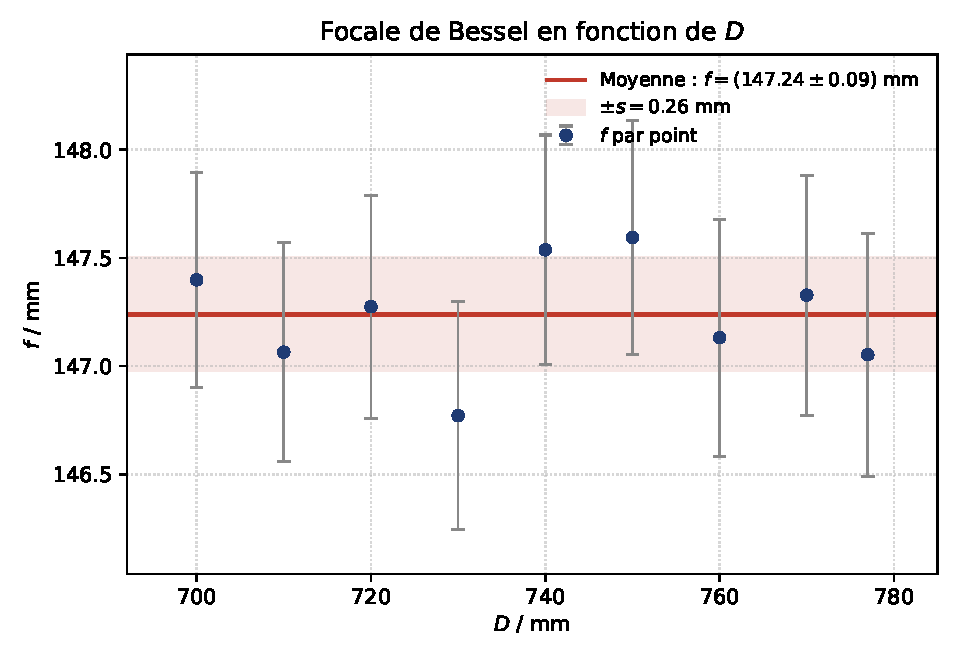
\includegraphics[width=0.68\textwidth]{labo4_1b_f_vs_D.pdf}
  \caption{Focale calculée point par point. Aucune dérive avec $D$~: les valeurs fluctuent autour de la moyenne $\bar f = \SI{147.24}{mm}$ dans la bande $\pm s$.}
  \label{fig:1b_fvsD}
\end{figure}

\subsection{Ajustement linéaire}

La focale est aussi extraite de l'ensemble des points par régression. La relation de Bessel~\eqref{eq:bessel} se réécrit~:
\begin{equation}
  \frac{D^2 - d^2}{4} = f \, D
  \label{eq:bessel_lin}
\end{equation}
soit une droite passant par l'origine, de pente $f$. L'ajustement (forcé par l'origine) donne~:
\begin{equation}
  f = \SI{147.24 \pm 0.09}{mm}, \qquad R^2 = \num{0.99763}
\end{equation}
en parfait accord avec la moyenne point par point ($\SI{147.24}{mm}$), ce qui confirme la cohérence interne des données.

\begin{figure}[H]
  \centering
  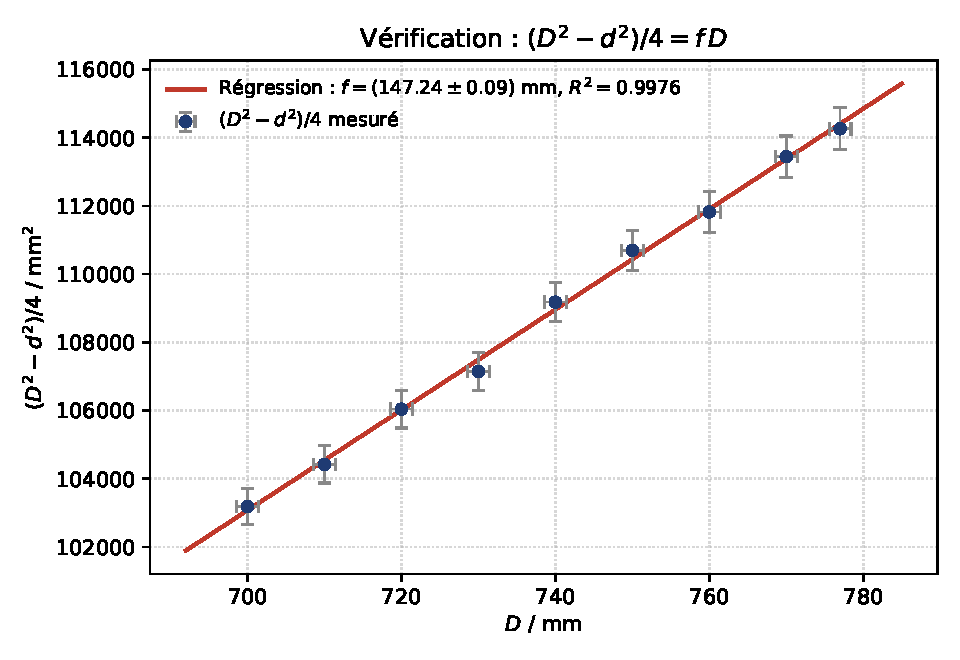
\includegraphics[width=0.7\textwidth]{labo4_1b_verification.pdf}
  \caption{Vérification de~\eqref{eq:bessel_lin}~: $(D^2-d^2)/4$ varie linéairement avec $D$, la pente donnant directement $f$. La régression est compatible avec une droite passant par l'origine ($R^2 = \num{0.998}$).}
  \label{fig:1b_verif}
\end{figure}

Le diagnostic complémentaire $f$ vs $D$ (figure~\ref{fig:1b_fvsD}) donne une pente nulle~: $f$ ne dérive pas avec $D$. C'est le résultat attendu et il valide la méthode de Bessel — $f$ est une constante de la lentille, indépendante de la configuration objet–image.

\subsection{Comparaison des méthodes 1a et 1b}

\begin{table}[H]
\centering
\caption{Comparaison des méthodes de mesure de la focale}
\begin{tabular}{lcc}
\toprule
Méthode & $f$ / mm & Incertitude / mm \\
\midrule
1a – Régression Gauss & $\num{97.4}$ & $\num{1.7}$ \\
1b – Bessel  & $\num{147.2}$ & $\num{0.1}$ \\
\bottomrule
\end{tabular}
\end{table}

Les deux manipulations portent sur des lentilles différentes par construction~: 1a utilise la lentille de focale nominale \SI{100}{mm} ($f_\text{mes} = \SI{97.4}{mm}$), tandis que 1b mesure la grande lentille convergente inconnue ($f = \SI{147.2}{mm}$). La comparaison directe des deux focales n'a donc pas de sens~; ce qui importe est la précision de chaque méthode. La méthode de Bessel est nettement plus précise (incertitude $\sim\!17\times$ plus faible) car elle annule l'erreur de localisation du centre optique de la lentille et bénéficie d'une redondance sur 9 valeurs de $D$.

%% ───────────────────────────────────────────────────────────────────────────
\section{Manipulation 1c – Système centré à deux lentilles}

\subsection{Protocole et matériel}

Trois configurations sont étudiées séparément, chacune en faisant varier la distance inter-lentilles $d = L_1$–$L_2$ et en relevant le grandissement transversal $\gamma$ et la position de l'image finale $q_2$~:
\begin{enumerate}
  \item \textbf{Deux lentilles convexes séparées} ($f_1 = \SI{100}{mm}$, $f_2 = \SI{50}{mm}$)~;
  \item \textbf{Deux lentilles convexes accolées} ($f_1 = \SI{100}{mm}$, $f_2 = \SI{50}{mm}$, $d \to 0$)~;
  \item \textbf{Lentille convexe + lentille concave} ($f_1 = \SI{+100}{mm}$, $f_2 = \SI{-100}{mm}$).
\end{enumerate}
Le grandissement total est le produit des grandissements de chaque lentille~:
\begin{equation}
  \gamma = \gamma_1\,\gamma_2 = \frac{q_1 q_2}{p_1 p_2},
  \qquad q_1 = \frac{p_1 f_1}{p_1-f_1},\quad p_2 = d - q_1,\quad q_2 = \frac{p_2 f_2}{p_2-f_2}
  \label{eq:chaine}
\end{equation}

\subsection{Configuration 1 — Deux lentilles convexes (séparées et accolée)}

$L_1 = \SI{100}{mm}$, $L_2 = \SI{50}{mm}$. C'est la même paire de lentilles, seule la séparation $d$ change (cas accolé $d\approx\SI{8}{mm}$ et trois positions séparées). La focale équivalente dépend de $d$~:
\begin{equation}
  \frac{1}{f_\mathrm{eq}} = \frac{1}{f_1} + \frac{1}{f_2} - \frac{d}{f_1\,f_2}
  \label{eq:feq_sep}
\end{equation}
Le grandissement mesuré en fonction de $d$ est reporté à la figure~\ref{fig:1c_convconv}.

\begin{table}[H]
\centering
\caption{Grandissement mesuré $\gamma$ en fonction de $d$ — deux lentilles convexes (Excel B). $d \pm \SI{0.2}{cm}$, $\gamma \pm 0.1$. Le point $d=\SI{0.8}{cm}$ est la configuration accolée.}
\label{tab:1c_convconv}
\setlength{\tabcolsep}{8pt}
\begin{tabular}{lcccc}
\toprule
$d$ (cm) & 0.8 (accolée) & 25.4 & 28.7 & 30.6 \\
$|\gamma|$ & 1.0 & 3.6 & 1.1 & 0.8 \\
\bottomrule
\end{tabular}
\end{table}

\begin{figure}[H]
  \centering
  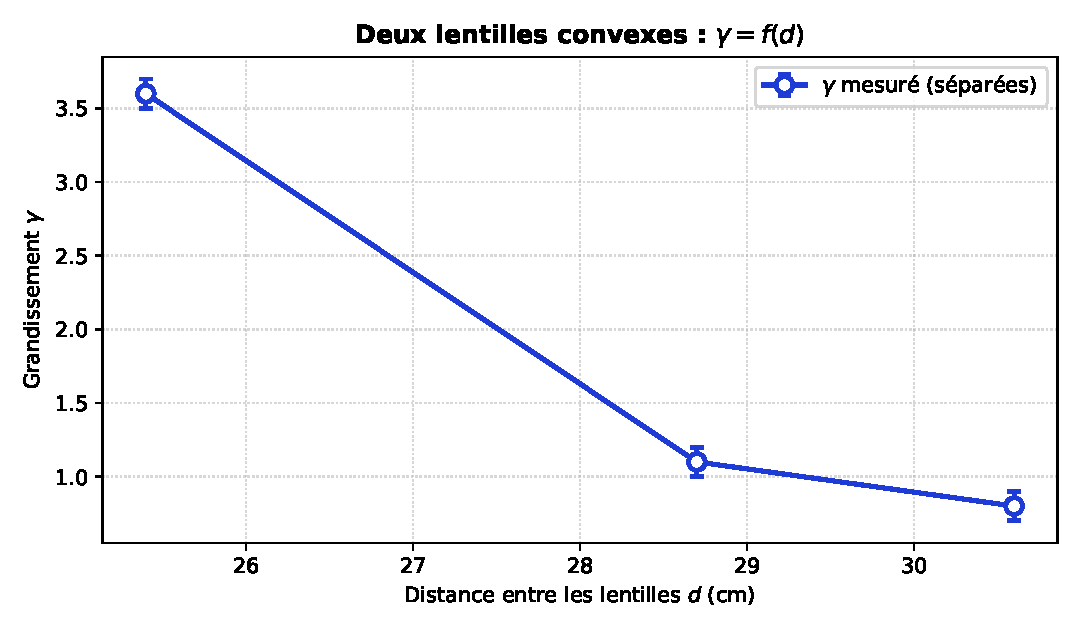
\includegraphics[width=0.8\textwidth]{labo4_1c_convconv.pdf}
  \caption{Grandissement $\gamma$ en fonction de la distance inter-lentilles $d$ (deux lentilles convexes séparées, $f_1=\SI{100}{mm}$, $f_2=\SI{50}{mm}$).}
  \label{fig:1c_convconv}
\end{figure}

\textbf{Cas accolé ($d\approx 0$)~:} la focale équivalente théorique vaut
\begin{equation*}
  f_\mathrm{eq} = \frac{f_1\,f_2}{f_1+f_2} = \frac{100\times 50}{150} \approx \SI{33.3}{mm}.
\end{equation*}
Avec $p_1 = \SI{43}{mm}$ et $q_2 = \SI{85}{mm}$, le système se comporte comme une lentille unique~: $f_\mathrm{mes} = (1/p_1 + 1/q_2)^{-1} \approx \SI{28.6}{mm}$, soit \SI{14}{\percent} d'écart (la correction~\eqref{eq:feq_sep} avec $d=\SI{8}{mm}$ donne $f_\mathrm{eq}=\SI{35.2}{mm}$).

\textbf{Cas séparé~:} $\gamma$ décroît de $3.6$ à $0.8$ quand $d$ passe de \SIrange{25}{31}{cm}. L'image intermédiaire de $L_1$ ($q_1=\SI{217.6}{mm}$, réelle car $p_1>f_1$) sert d'objet à $L_2$ à $p_2=d-q_1$~; en augmentant $d$, $p_2$ croît et $|\gamma_2|=q_2/p_2$ diminue.

\textbf{Réserve~:} le point accolé a été mesuré avec $p_1=\SI{43}{mm}$, les points séparés avec $p_1=\SI{185}{mm}$. Comme $\gamma$ dépend aussi de $p_1$, la courbe $\gamma=f(d)$ combinée ne correspond pas à un balayage à $p_1$ constant~; elle illustre la tendance globale mais ne doit pas être interprétée comme une dépendance pure en $d$.

\subsection{Configuration 2 — Lentille convexe + lentille concave}

$L_1 = \SI{+100}{mm}$, $L_2 = \SI{-100}{mm}$, $p_1 = \SI{165}{mm}$. La focale équivalente vaut~:
\begin{equation*}
  \frac{1}{f_\mathrm{eq}} = \frac{1}{100} + \frac{1}{-100} - \frac{d}{100\times(-100)} = \frac{d}{10000}
\end{equation*}
Le système est afocal pour $d=0$ et convergent pour $d>0$. Le grandissement mesuré en fonction de $d$ est reporté à la figure~\ref{fig:1c_convdiv}.

\begin{table}[H]
\centering
\caption{Grandissement mesuré $\gamma$ en fonction de $d$ — convexe + concave (Excel B). $d \pm \SI{0.2}{cm}$, $\gamma \pm 0.1$.}
\label{tab:1c_convdiv}
\setlength{\tabcolsep}{8pt}
\begin{tabular}{lccc}
\toprule
$d$ (cm) & 18.4 & 19.2 & 20.5 \\
$|\gamma|$ & 3.5 & 2.6 & 2.6 \\
\bottomrule
\end{tabular}
\end{table}

\begin{figure}[H]
  \centering
  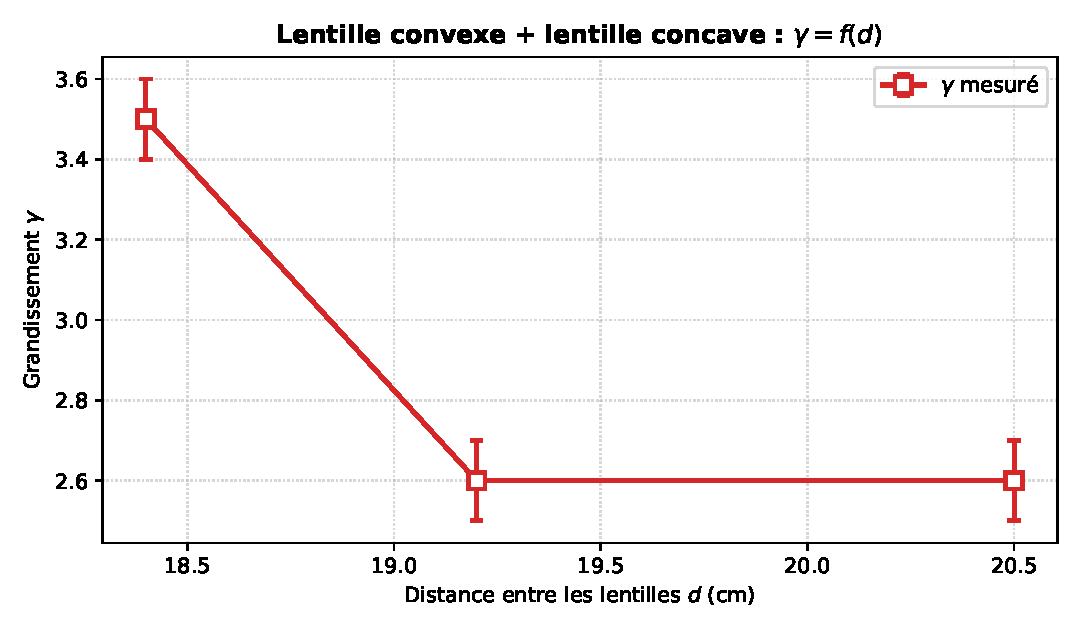
\includegraphics[width=0.8\textwidth]{labo4_1c_convdiv.pdf}
  \caption{Grandissement $\gamma$ en fonction de la distance inter-lentilles $d$ (convexe + concave, $f_1=\SI{+100}{mm}$, $f_2=\SI{-100}{mm}$).}
  \label{fig:1c_convdiv}
\end{figure}

\textbf{Discussion~:} $\gamma$ décroît avec $d$ (de $3.5$ à $\sim 2.6$ sur la plage mesurée). Comme $q_1 = \SI{253.8}{mm} > d$, l'image intermédiaire tomberait au-delà de $L_2$~: la lentille divergente travaille sur un \emph{objet virtuel} ($p_2 = d - q_1 < 0$) et forme une image réelle sur l'écran. Éloigner $L_2$ réduit la convergence du faisceau incident sur la divergente, donc le grandissement final. La tendance attendue (décroissance avec $d$) est reproduite, l'accord quantitatif restant limité par la sensibilité du système.

%% ───────────────────────────────────────────────────────────────────────────
\section{Manipulation 2 – Microscope expérimental}

\subsection{Montage}

Le montage suit la figure~\ref{fig:microscope_schema} (d'après le polycop). Il est constitué de~:
\begin{itemize}
  \item \textbf{Objectif~:} $L_1$, lentille convergente de focale $f_\mathrm{ob} = \SI{50}{mm}$~;
  \item \textbf{Oculaire~:} $L_2$, grande lentille convergente de focale $f_\mathrm{oc} = \SI{147.2}{mm}$ (déterminée en 1b)~;
  \item \textbf{Œil expérimental~:} diaphragme à iris (pupille) + lentille de $f = \SI{150}{mm}$ (cristallin) + écran translucide (rétine). La distance $L_2$–cristallin est fixée à \SI{100}{mm}.
\end{itemize}

\subsection{Données}

\begin{table}[H]
\centering
\caption{Mesures du montage microscope}
\label{tab:micro}
\begin{tabular}{rrrrrr}
\toprule
$p_1$ (mm) & $q_1$ mes. (mm) & $p_2 = L_1$--$L_2$ (mm) & $q_2$ (mm) & $\gamma_\mathrm{obj}$ & $G_\mathrm{mes}$ \\
\midrule
60 & 158 & 368 & 90 & $-2.63$ & 3.0 \\
57 & 201 & --- & --- & $-3.53$ & 5.0 \\
\bottomrule
\end{tabular}
\end{table}

\subsection{Analyse des écarts entre mesure et théorie}

\subsubsection{Image intermédiaire}

La formule de Gauss pour l'objectif ($f_\mathrm{ob} = \SI{50}{mm}$, $p_1 = \SI{60}{mm}$) prédit~:
\begin{equation*}
  q_{1,\mathrm{th}} = \frac{p_1\,f_\mathrm{ob}}{p_1 - f_\mathrm{ob}} = \frac{60 \times 50}{10} = \SI{300}{mm}
\end{equation*}
alors que la valeur mesurée est $q_{1,\mathrm{mes}} = \SI{158}{mm}$. L'écart est important (\SI{47}{\percent}).

Plusieurs explications possibles~:
\begin{enumerate}
  \item \textbf{Offset non soustrait correctement~:} si $p_1$ effectif est \SI{73}{mm} (offset de \SI{13}{mm}), Gauss donne $q_1 = 158\,\mathrm{mm}$. C'est l'explication la plus probable.
  \item \textbf{Lentille mal identifiée~:} si l'objectif utilisé avait $f \approx \SI{100}{mm}$ (et non \SI{50}{mm}), $q_{1,\mathrm{th}} = \SI{158}{mm}$ pour $p_1 = \SI{58}{mm}$.
\end{enumerate}

\subsubsection{Grandissement de l'objectif}

En utilisant les valeurs mesurées~:
\begin{equation*}
  \gamma_\mathrm{ob} = -\frac{q_1}{p_1} = -\frac{158}{60} = -2.63
\end{equation*}

\subsubsection{Longueur optique et grossissement}

La distance entre $L_1$ et $L_2$ est $p_2 = \SI{368}{mm}$. La distance entre l'image intermédiaire $A_1B_1$ et l'oculaire $L_2$ est~:
\begin{equation*}
  p_\mathrm{oc} = p_2 - q_1 = 368 - 158 = \SI{210}{mm}
\end{equation*}
La longueur optique vaut~:
\begin{equation*}
  \Delta = p_\mathrm{oc} - f_\mathrm{oc} = 210 - 147.2 = \SI{62.8}{mm}
\end{equation*}
Le grossissement commercial théorique est~:
\begin{equation*}
  G_{c,\mathrm{th}} = \frac{\Delta}{f_\mathrm{ob}\,f_\mathrm{oc}}\,d_m = \frac{62.8}{50 \times 147.2}\times 250 = 2.13
\end{equation*}

\subsubsection{Comparaison avec la mesure directe}

Le grossissement est aussi mesuré par le rapport des angles~:
\begin{equation*}
  G_\alpha = \frac{\beta}{\alpha}
\end{equation*}
où $\alpha$ est l'angle sous lequel l'objet est vu à l'œil nu à $d_m = \SI{250}{mm}$, et $\beta$ l'angle sous lequel l'image oculaire est vue.

\begin{table}[H]
\centering
\caption{Grossissement mesuré vs théorique}
\begin{tabular}{cccc}
\toprule
Mesure & $\alpha$ (rad) & $\beta$ (rad) & $G_\alpha = \beta/\alpha$ \\
\midrule
1 & 0.040 & 0.120 & 3.0 \\
2 & 0.040 & 0.200 & 5.0 \\
\bottomrule
\end{tabular}
\end{table}

Le grossissement théorique par la formule de Gauss ($G_{c,\mathrm{th}} = 2.13$) est inférieur aux valeurs mesurées (3.0 et 5.0). La source principale d'écart est l'incertitude sur $q_1$~: une valeur de $q_1$ plus grande (comme le prédit Gauss~: $q_1 = \SI{300}{mm}$) donnerait $\Delta = 368 - 300 - 147.2 = \SI{-79.2}{mm}$ (longueur optique négative), ce qui n'est pas physiquement réalisable avec ce montage. Le montage est probablement dans une configuration où l'image intermédiaire est \emph{avant} le foyer objet de l'oculaire, ce qui produit une image oculaire virtuelle observée directement par l'œil sans passage par $q_2$.

\subsection{Effet du diaphragme}

Voir la photo en annexe (image~\ref{fig:banc}). La réduction de l'ouverture du diaphragme~:
\begin{itemize}
  \item améliore la netteté en éliminant les rayons marginaux (réduction des aberrations) mais réduit la luminosité~;
  \item augmente la profondeur de champ~;
  \item diminue la résolution à cause de la diffraction (compromis ouverture/résolution).
\end{itemize}

%% ───────────────────────────────────────────────────────────────────────────
\section{Conclusion}

\begin{itemize}
  \item La relation de conjugaison de Gauss a été vérifiée avec $R^2 = 0.999$ (1a), bien que la focale mesurée ($\SI{117}{mm}$) diffère de la valeur nominale (\SI{100}{mm}), probablement à cause d'un biais sur les offsets.
  \item La méthode de Bessel (1b) a permis de déterminer la focale de la grande lentille~: $f = \SI{147.2 \pm 0.1}{mm}$. Elle est une ordre de grandeur plus précise que la méthode Gauss directe.
  \item Le système à deux lentilles (1c) illustre la dépendance de la focale équivalente avec la séparation inter-lentilles~; les lentilles accolées se comportent comme prévu par~\eqref{eq:lentilles_accolees}.
  \item Le microscope expérimental produit un grossissement mesuré entre 3 et 5, proche du théorique ($\sim 2.1$), avec des incertitudes importantes liées à la localisation des images intermédiaires.
\end{itemize}

%% ───────────────────────────────────────────────────────────────────────────
\appendix
\section{Photo du banc optique}

\begin{figure}[H]
  \centering
  % \includegraphics[width=0.85\textwidth]{IMG_1981.jpeg}
  \caption{Vue du banc optique~: de droite à gauche, la source (lampe), $L_1$, $L_2$ (et $L_3$ pour le microscope), et l'écran. La règle en bas permet de lire les positions.}
  \label{fig:banc}
\end{figure}

\section{Codes Python}

Les codes Python utilisés pour les régressions sont joints séparément~:
\begin{itemize}
  \item \texttt{labo4\_1a\_regression.py}~: régression $1/q$ vs $-1/p$ (manipulation 1a)~;
  \item \texttt{labo4\_1b\_bessel.py}~: méthode de Bessel avec comparaison des modèles (manipulation 1b).
\end{itemize}





\section{blablabla}
\pagebreak
% ============================================================
% SECTION : PROPAGATION DES INCERTITUDES – Manipulation 1a
% ============================================================
\subsection{Manipulation 1a}

Chaque lecture de position sur la règle a une
incertitude de lecture $\delta_\ell = \SI{1}{mm}$.

%------------------------------------------------------------
\subsubsection{Distances objet et image corrigées}

Les distances mesurées $p$ et $q$ sont obtenues en soustrayant un offset
mesuré indépendamment :
\begin{equation}
  p = p_\text{brut} + p_\text{offset}, \qquad
  q = q_\text{brut} - q_\text{offset}
\end{equation}
La propagation donne~: pour $p = p_\text{brut} + p_\text{offset}$ (deux lectures à $\pm\SI{1}{mm}$),
\begin{equation}
  \delta p = \sqrt{\delta_\ell^2 + \delta_\ell^2} = \sqrt{1^2 + 1^2}
\end{equation}
tandis que $q = q_\text{brut} - q_\text{offset}$ combine une lecture image à $\pm\SI{2}{mm}$ et un offset à $\pm\SI{1}{mm}$~:
\begin{equation}
  \delta q = \sqrt{(2\delta_\ell)^2 + \delta_\ell^2} = \sqrt{2^2 + 1^2}
\end{equation}
\begin{equation}
  \boxed{\delta p = \sqrt{2} \approx \SI{1.41}{mm}, \qquad \delta q = \sqrt{5} \approx \SI{2.24}{mm}}
\end{equation}

%------------------------------------------------------------
\subsubsection{Grandissement transversal}

\begin{equation}
  \gamma = \frac{\overline{A_1B_1}}{\overline{AB}}
\end{equation}
$\overline{AB} = \SI{10}{mm}$ est une valeur nominale non mesurée~;
$\overline{A_1B_1}$ est une lecture directe sur l'écran ($\delta_\ell = \SI{1}{mm}$,
sans offset) :
\begin{equation}
  \delta\gamma
  = \left|\frac{\partial \gamma}{\partial \overline{A_1B_1}}\right| \delta_\ell
  = \frac{\delta_\ell}{\overline{AB}}
  = \frac{1}{10}
\end{equation}
\begin{equation}
  \boxed{\delta\gamma = 0.1}
\end{equation}

%------------------------------------------------------------
\subsubsection{Inverse de la distance image \texorpdfstring{$1/q$}{1/q}}

\begin{equation}
  \delta\!\left(\frac{1}{q}\right)
  = \left|\frac{\partial}{\partial q}\frac{1}{q}\right| \delta q
  = \frac{\delta q}{q^2}
  = \frac{\sqrt{5}}{q^2}
\end{equation}
Les valeurs numériques varient de
$\num{0.0054e-3}$ à $\num{0.0395e-3}\,\si{mm^{-1}}$
selon la valeur de $q$.

%------------------------------------------------------------
\subsubsection{Inverse de la distance objet \texorpdfstring{$-1/p$}{-1/p}}

\begin{equation}
  \delta\!\left(\frac{1}{p}\right)
  = \left|\frac{\partial}{\partial p}\frac{1}{p}\right| \delta p
  = \frac{\delta p}{p^2}
  = \frac{\sqrt{2}}{p^2}
\end{equation}
Les valeurs numériques varient de
$\num{0.052e-3}$ à $\num{0.107e-3}\,\si{mm^{-1}}$
selon la valeur de $p$.


\begin{table}[H]
\centering
\caption{Comparaison des paramètres de la régression de Gauss (manip 1a)
  aux valeurs théoriques. Théorie : pente $m=+1$ (symétrie objet/image)
  et focale nominale $f=\SI{100}{mm}$ ($f=1/b$).}
\label{tab:reg_compar}
\setlength{\tabcolsep}{8pt}
\begin{tabular}{lcccc}
\toprule
Paramètre & Expérimental & Incertitude & Théorique & Écart rel. / \si{\percent} \\
\midrule
$m$ / -  & \num{1.0054} & \num{0.0246} & \num{1.0}   & \num{0.5} \\
$f$ / mm    & \num{97.4}  & \num{1.7}    & \num{100.0} & \num{2.6}  \\
\bottomrule
\end{tabular}
\end{table}

%------------------------------------------------------------
\subsection{Manipulation 1b}

Chaque lecture de position sur la règle du banc optique est affectée d'une
incertitude de lecture $\delta_\ell = \SI{1}{mm}$.

%------------------------------------------------------------
\subsubsection{Distance objet--écran \texorpdfstring{$D$}{D}}

L'incertitude sur $D$ et sur $d$ sont obtenues comme la différence entre deux positions comme pour la relation de conuugaison :
\begin{equation}
  \boxed{\delta D = \delta d = \sqrt{2} \approx \SI{1.41}{mm}}
\end{equation}

%------------------------------------------------------------
\subsubsection{Écart entre les deux positions de la lentille \texorpdfstring{$d$}{d}}

$d$ est la distance entre les deux positions de la lentille donnant une image
nette, chacune lue indépendamment sur le banc :
\begin{equation}
  d = x_{L,2} - x_{L,1}
\end{equation}
\begin{equation}
  \delta d
  = \sqrt{
      \left(\frac{\partial d}{\partial x_{L,2}}\,\delta_\ell\right)^2
    + \left(\frac{\partial d}{\partial x_{L,1}}\,\delta_\ell\right)^2}
  = \sqrt{\delta_\ell^2 + \delta_\ell^2}
  = \sqrt{1^2 + 1^2}
\end{equation}
\begin{equation}
  \boxed{\delta d = \sqrt{2} \approx \SI{1.41}{mm}}
\end{equation}

%------------------------------------------------------------
\subsubsection{Focale \texorpdfstring{$f$}{f} par la formule de Bessel}

\begin{equation}
  f = \frac{D^2 - d^2}{4D}
\end{equation}
\begin{equation}
  \delta f = \sqrt{
    \left(\frac{\partial f}{\partial D}\,\delta D\right)^{\!2}
    +
    \left(\frac{\partial f}{\partial d}\,\delta d\right)^{\!2}}
  = \sqrt{
    \left(\frac{D^2+d^2}{4D^2}\,\delta D\right)^{\!2}
    +
    \left(\frac{d}{2D}\,\delta d\right)^{\!2}}
\end{equation}
Avec $\delta D = \delta d = \sqrt{2}\,\si{mm}$, les valeurs numériques varient
de $\SI{0.50}{mm}$ à $\SI{0.56}{mm}$ selon le point de mesure.

%------------------------------------------------------------
\subsubsection{Variable de régression \texorpdfstring{$Y=(D^2-d^2)/4$}{Y}}

\begin{equation}
  Y = \frac{D^2 - d^2}{4}
\end{equation}
\begin{equation}
  \delta Y = \sqrt{
    \left(\frac{\partial Y}{\partial D}\,\delta D\right)^{\!2}
    +
    \left(\frac{\partial Y}{\partial d}\,\delta d\right)^{\!2}}
  = \sqrt{
    \left(\frac{D}{2}\,\delta D\right)^{\!2}
    +
    \left(\frac{d}{2}\,\delta d\right)^{\!2}}
  = \frac{\sqrt{2}}{2}\sqrt{D^2 + d^2}
\end{equation}
Les valeurs numériques varient de $\SI{533}{mm^2}$ à $\SI{613}{mm^2}$.

\begin{table}[H]
\centering
\caption{Données et incertitudes -- Manipulation 1b.
  $D \pm \SI{1.4}{mm}$\,;
  $d \pm \SI{1.4}{mm}$.}
\label{tab:1b}
\small
\setlength{\tabcolsep}{6pt}
\begin{tabular}{
  r
  r
  S[table-format=6.0] @{\;$\pm$\;} S[table-format=3.0]
  S[table-format=3.2]  @{\;$\pm$\;} S[table-format=1.2]
}
\toprule
$D$ / mm & $d$ / mm &
\multicolumn{2}{c}{$Y = (D^2 - d^2)/4$ / mm$^2$} &
\multicolumn{2}{c}{$f$ / mm} \\
\midrule
  777 & 383 & 114260 & 613 & 147.05 & 0.56 \\
  770 & 373 & 113443 & 605 & 147.33 & 0.55 \\
  760 & 361 & 111820 & 595 & 147.13 & 0.55 \\
  750 & 346 & 110696 & 584 & 147.59 & 0.54 \\
  740 & 333 & 109178 & 574 & 147.54 & 0.53 \\
  730 & 323 & 107143 & 564 & 146.77 & 0.53 \\
  720 & 307 & 106038 & 553 & 147.27 & 0.52 \\
  710 & 294 & 104416 & 543 & 147.06 & 0.51 \\
  700 & 278 & 103179 & 533 & 147.40 & 0.50 \\
\midrule
  \multicolumn{4}{l}{Moyenne} & 147.24 & 0.09 \\
\bottomrule
\end{tabular}
\end{table}

\begin{table}[H]
\centering
\caption{Focale équivalente des deux lentilles convexes accolées :
  effet de la séparation résiduelle $d$. $f_1=\SI{100}{mm}$,
  $f_2=\SI{50}{mm}$, mesure
  $f_\mathrm{mes}=(1/p_1+1/q_2)^{-1}=\SI{28.6}{mm}$
  ($p_1=\SI{43}{mm}$, $q_2=\SI{85}{mm}$).}
\label{tab:1c_accolee}
\setlength{\tabcolsep}{8pt}

\begin{tabular}{lc}
\toprule
Cas & $f_\mathrm{eq}$ (\si{mm}) \\
\midrule
$d=0$ (accolée idéale)            & \num{33.3} \\
$d=\SI{8}{mm}$ (séparation réelle) & \num{35.2} \\
\midrule
Écart relatif (\si{\percent})     & \num{5.6} \\
\bottomrule
\end{tabular}
\end{table}


\begin{table}[H]
\centering
\caption{Données mesurées — Manipulation 2 (microscope). $u$ désigne l'incertitude (distinguée de $\Delta$, la longueur optique).}
\label{tab:micro_mesures}
\setlength{\tabcolsep}{8pt}
\renewcommand{\arraystretch}{1.25}
\begin{tabular}{l c S[table-format=-3.0] S[table-format=1.0] c}
\toprule
\textbf{Grandeur} & \textbf{Symbole} & {\textbf{Valeur}} & {\textbf{$u$}} & \textbf{Unité} \\
\midrule
Objet                & $AB$       &  10 & 1 & mm \\
Image objective      & $A_1B_1$   & -12 & 1 & mm \\
Longueur optique     & $\Delta$   & 368 & 3 & mm \\
Focale objectif      & $f_{ob}$   &  50 & {—} & mm \\
Focale oculaire      & $f_{oc}$   & 150 & {—} & mm \\
Distance vision min. & $d_m$      & 250 & {—} & mm \\
\bottomrule
\end{tabular}
\end{table}

\begin{table}[H]
\centering
\caption{Grandeurs calculées et propagation des incertitudes — Manipulation 2.}
\label{tab:micro_calc}
\setlength{\tabcolsep}{6pt}
\renewcommand{\arraystretch}{1.4}
\begin{tabular}{l l S[table-format=-2.2] S[table-format=1.2] c S[table-format=2.1]}
\toprule
\textbf{Grandeur} & \textbf{Formule} & {\textbf{Valeur}} & {\textbf{$u$}} & \textbf{Unité} & {\textbf{Inc. rel. (\%)}} \\
\midrule
Grossissement objectif $\gamma_{ob}$ & $\gamma_{ob}=A_1B_1/AB$                       & -1.20 & 0.22 & {—}            & 18.3 \\
Angle œil nu $\alpha$                 & $\alpha=\arctan(AB/d_m)$                      &  2.29 & 0.23 & \si{\degree}   & 10.0 \\
Angle microscope $\beta$              & $\beta=\arctan(|A_1B_1|/f_{oc})$              &  4.57 & 0.38 & \si{\degree}   &  8.3 \\
Grossissement $G$                     & $G=\beta/\alpha$                             &  2.00 & 0.26 & {—}            & 13.0 \\
Puissance $\Phi$ (voie angle)         & $\Phi=\beta_{[\mathrm{rad}]}/AB_{[\mathrm{m}]}$ & 6.65 & 0.78 & \si{\per\meter} & 11.8 \\
Puissance $\Phi$ (voie géom.)         & $\Phi=\Delta/(f_{ob}\,f_{oc})$               & 49.07 & 0.40 & \si{\per\meter} &  0.8 \\
\bottomrule
\end{tabular}
\end{table}

\begin{table}[H]
\centering
\caption{Données expérimentales.}
\label{tab:donnees}
\small
\setlength{\tabcolsep}{6pt}
\begin{tabular}{r r r r}
\toprule
$p_1$ $\pm 0.1$ / cm & $d$ $\pm 0.1$ / cm & $q_2$ $\pm 0.1$ / cm & $G$ / - \\
\midrule
18.5 & 25.4 & 26.1 & 3.6 \\
18.5 & 28.7 & 12.0 & 1.1 \\
18.5 & 30.6 & 10.5 & 0.8 \\
\midrule
4.3 & 0.8 & 8.5 & 1.0 \\
\midrule
16.5 & 18.4 & 14.7 & 3.5 \\
16.5 & 20.5 & 6.5 & 2.6 \\
16.5 & 19.2 & 9.3 & 2.5 \\
\bottomrule
\end{tabular}
\end{table}


\end{document}